%%%%%%%%%%%%%%%%%%%%%%%%%%%%%%%%%%%%%%%%%
% University/School Laboratory Report
% LaTeX Template
% Version 3.1 (25/3/14)
%
% This template has been downloaded from:
% http://www.LaTeXTemplates.com
%
% Original author:
% Linux and Unix Users Group at Virginia Tech Wiki 
% (https://vtluug.org/wiki/Example_LaTeX_chem_lab_report)
%
% License:
% CC BY-NC-SA 3.0 (http://creativecommons.org/licenses/by-nc-sa/3.0/)
%
%%%%%%%%%%%%%%%%%%%%%%%%%%%%%%%%%%%%%%%%%

%----------------------------------------------------------------------------------------
%	PACKAGES AND DOCUMENT CONFIGURATIONS
%----------------------------------------------------------------------------------------

\documentclass{article}

\usepackage[version=3]{mhchem} % Package for chemical equation typesetting
\usepackage{siunitx} % Provides the \SI{}{} and \si{} command for typesetting SI units
\usepackage{graphicx} % Required for the inclusion of images
\usepackage{natbib} % Required to change bibliography style to APA
\usepackage{amsmath} % Required for some math elements 
\usepackage[utf8]{inputenc}
\usepackage[margin=1.2in]{geometry}
\usepackage{hyperref}

\setlength\parindent{0pt} % Removes all indentation from paragraphs

% \renewcommand{\labelenumi}{\alph{enumi}.} % Make numbering in the enumerate environment by letter rather than number (e.g. section 6)

\renewcommand{\figurename}{Figura}
\renewcommand{\tablename}{Tabla}
\renewcommand\refname{Referencias}

\def\mean#1{\left< #1 \right>}
%\usepackage{times} % Uncomment to use the Times New Roman font

%----------------------------------------------------------------------------------------
%	DOCUMENT INFORMATION
%----------------------------------------------------------------------------------------

\title{M\'etodos num\'ericos para la Ciencia e Ingenier\'ia \\ Tarea 11: Ajuste de Curvas Bayesiano} % Title

\author{Felipe Toledo B.} % Author name

\date{\today} % Date for the report

\begin{document}

\maketitle % Insert the title, author and date

%----------------------------------------------------------------------------------------
%	SECTION 1
%----------------------------------------------------------------------------------------

\section{Introducción}

En el presente trabajo se estudian modelos orientados a describir una línea de absorción de una observación espectroscópica, presentada en la Figura \ref{fig:datos_originales}.

\begin{figure}[ht]
  \centering
  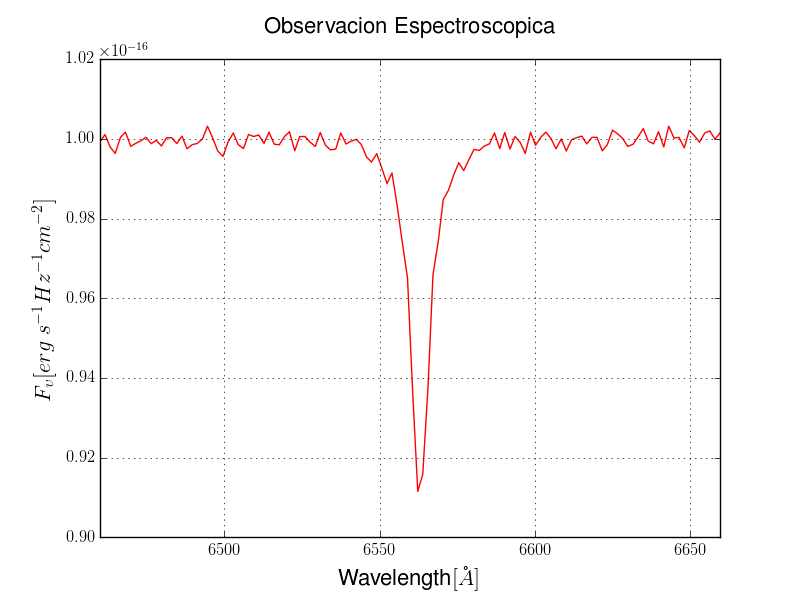
\includegraphics[scale = 0.55]{images/datos_originales.png}
  \caption{Datos originales observados. El nivel del continuo y la longitud de onda central de la línea de absorción son conocidos, con valores $1\cdot 10^{-16} [\frac{erg}{s\ Hz\ cm^{-2}}]$ y $6563[\AA]$ respectivamente.}
  \label{fig:datos_originales}
\end{figure}

Para describir la línea se probarán dos modelos:

\begin{itemize}

\item Línea Gaussiana Simple: A partir de la curva se observa que puede resultar conveniente describirla asumiendo que es de forma Gaussiana. En la ecuación (\ref{ec:modelo_1}) se explicita el modelo propuesto. 

\begin{equation}
f_1(\lambda) = C_0 - A e^{\frac{(\lambda - \mu_0)^2}{b}}
\label{ec:modelo_1}
\end{equation}

Éste posee dos parámetros libres, $A$ y $b$. El valor de $\mu_0$ y $C_0$ se asume conocido, donde $\mu_0$ es la longitud de onda central de la línea de absorción y $C_0$ corresponde al nivel del continuo.  

\item Línea Gaussiana Doble: El modelo está explicitado en la ecuación (\ref{ec:modelo_2}). Se tienen los mismos parámetros conocidos $\mu_0$ y $C_0$, pero en éste hay cuatro parámetros libres: $A_1$, $A_2$, $b_1$, $b_2$.

\begin{equation}
f_2(\lambda) = C_0 - A_1 e^{\frac{(\lambda - \mu_0)^2}{b_1}} - A_2 e^{\frac{(\lambda - \mu_0)^2}{b_2}}
\label{ec:modelo_2}
\end{equation}
\end{itemize}

Los objetivos son estimar el valor de cada parámetro con un intervalo de credibilidad del 68\%, usando métodos Bayesianos , y luego utilizar métodos de selección Bayesiana de modelos para decidir cuál de los dos propuestos representa mejor los datos.

\section{Metodología}



\subsection{Cálculo con Supernovas}
\label{sec:supernovas}

En ésta Sección se estima el valor de $H_0$ usando datos de Super Novas tipo I\footnote{Freedman et al. 2000}. Con ellas se pueden medir distancias muy superiores respecto al método de las Cefeidas. La regresión para este caso puede verse en la Figura \ref{fig:regresion_supernovas}, a partir de la cual se estima $H_0 = 70.7 [\frac{km}{Mpc \cdot s}]$. El valor obtenido es muy cercano al aceptado en la actualidad por la NASA\footnote{Publicado en su sitio web \url{http://map.gsfc.nasa.gov/universe/bb_tests_exp.html}}.

\begin{figure}[ht]
  \centering
  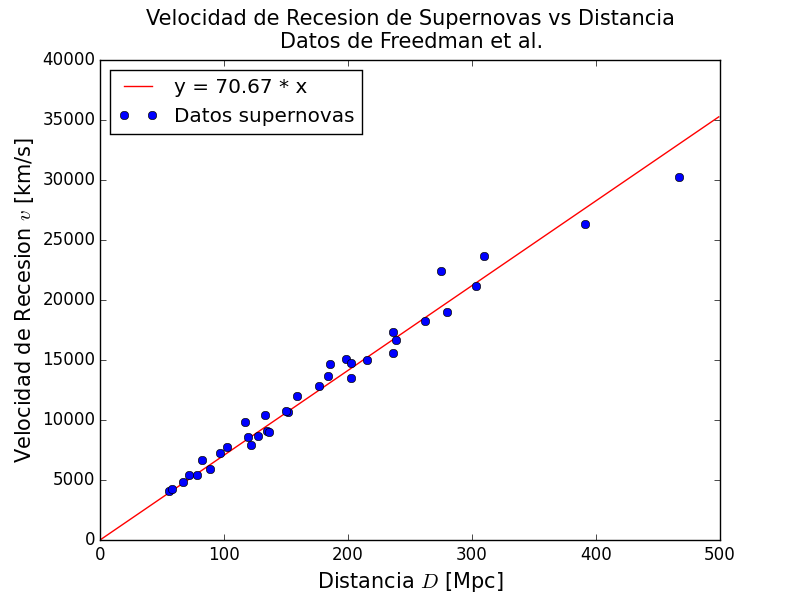
\includegraphics[scale = 0.55]{images/regresion_supernovas.png}
  \caption{Regresión para datos de Supernovas tipo I.}
  \label{fig:regresion_supernovas}
\end{figure}

Para el intervalo de confianza de 95\% se realiza una simulación Bootstrap análoga al caso de las Cefeidas, obteniéndose el histograma de la Figura \ref{fig:bootstrap_supernovas}. Según esta los valores de $H_0$ con un 95\% de confianza están entre 46 y 67 $[\frac{km}{Mpc \cdot s}]$.

\begin{figure}[ht]
  \centering
  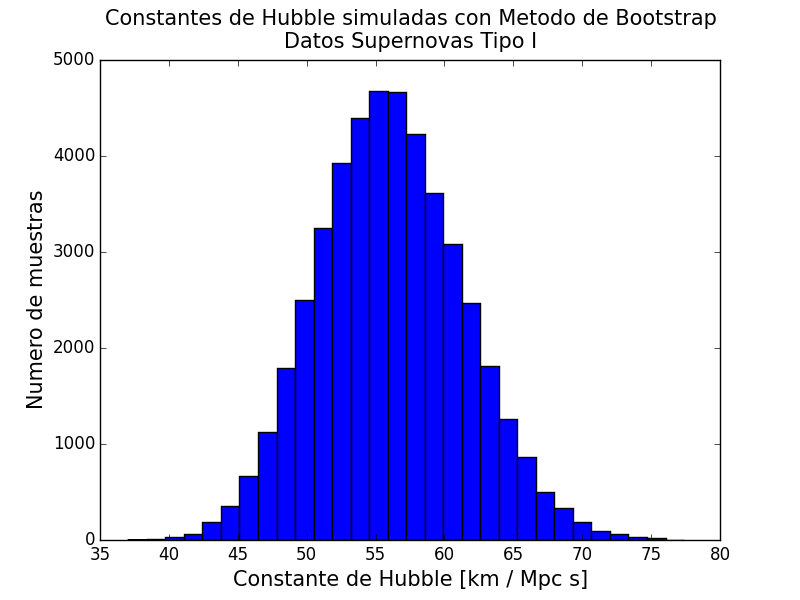
\includegraphics[scale = 0.55]{images/bootstrap_supernovas.png}
  \caption{Histograma con valores de $H_0$ generados usando Bootstrap. La cantidad de muestras en esta simulación es $100 N (\log{N})^2$, con $N=36$.}
  \label{fig:bootstrap_supernovas}  
\end{figure}

\subsection{Conclusiones}

Las regresiones muestran que para obtener datos de buena calidad es necesario tener muchas mediciones, o alternativamente, pocas mediciones de muy buena calidad. Se infiere de los resultados que los datos de las Supernovas son de mejor calidad que los de Cefeidas, ya que el valor de $H_0$ resultó mucho más cercano al aceptado y ambos disponían de una cantidad similar de datos. Esto último es razonable recordando que los datos de Supernovas se recolectaron casi cien años después, con todos los avances tecnológicos que ello conlleva.

En cuanto al método de Bootstrap, en ambas simulaciones indicó que los valores estimados a partir de mediciones reales quedan fuera del intervalo de confianza, implicando que son muy improbables. Para el caso de las Supernovas sabemos que el valor es correcto, por lo que se debe estudiar con detención donde está el problema. Bootstrap presume que no hay correlación entre la medición de un punto y el siguiente. Este enfoque funciona bien al tener una muestra de comportamiento poco correlacionado, como por ejemplo encuestas. En este problema, hay una evidente correlación entre distancia y velocidad. Como el método de Bootstrap no la considera, genera valores de comportamiento diferente a la muestra original, entregando intervalos de confianza anómalos.

\clearpage
\section{Intervalos de confianza Ajuste Lineal}

\subsection{Introducción}

Se dispone de un set de datos obtenidos del catálogo de cuasares \emph{Data Release 9} del \emph{Sloan Digital Sky Survey (SDSS)}. El objetivo de esta Sección es encontrar la recta que mejor modela la relación entre el flujo de la banda i y la banza z, encontrando el intervalo de confianza al 95\% para sus parámetros. 

Como el catálogo incluye valores del error para sus mediciones, se opta por utilizar una simulación de Monte Carlo con distribución de datos Gaussiana para encontrar el intervalo de confianza de los parámetros de la recta.

\subsection{Desarrollo}

Primero se observa la distribución de los datos para ver si efectivamente tienen tendencia lineal. En la Figura \ref{fig:datos_originales} se presentan los datos originales del catálogo, graficados uno vs el otro.


De la Figura se desprende que la mayoría de los datos están agrupados, con unos pocos datos lejos del grupo. Se podría implementar un filtro para eliminarlos del espacio muestral, pero como se desea estudiar el intervalo de confianza real se mantendrán durante el procesamiento.

\begin{figure}[ht]
  \centering
  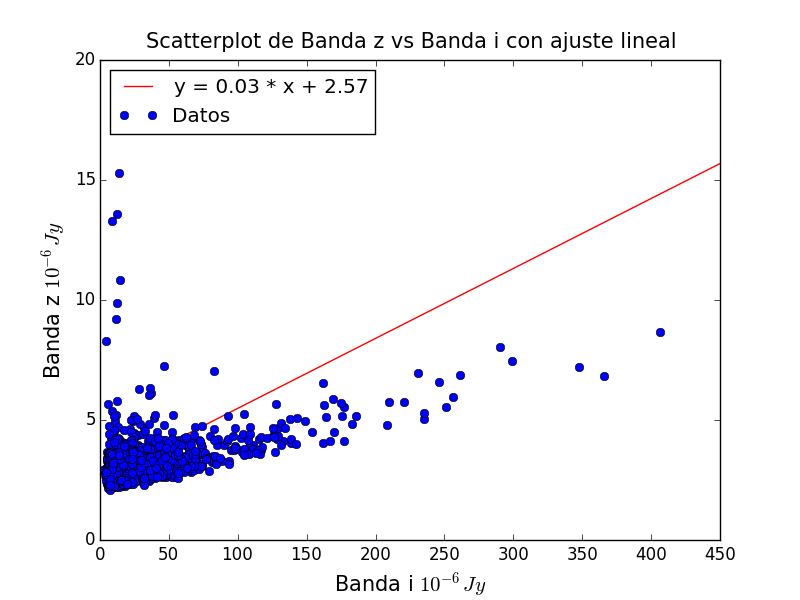
\includegraphics[scale=0.5]{images/datos_fit.png}
  \caption{Ajuste de los datos. Se ha realizado un zoom a la zona con mayor concentración de mediciones pero no se han eliminado datos del espacio muestral original.}
  \label{fig:datos_fit}
\end{figure}

Los parámetros encontrados para el ajuste $ banda_z(x) = a \cdot banda_i + b$ son $a = 0.03 \cdot 10^{-6}[Jy]$ y $b=2.57$. La regresión lineal se realizó usando la herramienta \emph{polyfit} de \emph{numpy}. Los valores obtenidos usando el método de Monte Carlo se presentan en la Tabla \ref{tab:montecarlo}.

\begin{table}[ht]
  \centering
  \begin{tabular}{|c|c|c|}
    \hline
    Variable & Min. Valor & Max. Valor \\
    \hline
    a [$10^{-6}Jy$] & 1.65 & 3.28\\
    \hline
    b & -0.005 & 0.067\\
    \hline 
  \end{tabular}
  \caption{Intervalos de confianza al 95\% para parámetros del ajuste lineal. Estimados con simulación de Monte Carlo de $10^4$ espacios muestrales, usando distribución Gaussiana con error conocido para la generación de datos.}
  \label{tab:montecarlo}
\end{table}

\section{Conclusiones}
En esta ocasión la estimación de los intervalos de confianza resultó ser más razonable que en el caso de la Constante de Hubble. El motivo por el que ello ocurre es que el método de Montecarlo preserva gran parte de la correlación entre los datos, ya que las muestras son creadas generando variaciones en torno a los valores originales. Aún más, como las variaciones en este caso son Gaussianas, su media es cero por lo que para una gran cantidad de simulaciones se espera que su valor medio coindica con el ajuste lineal de las mediciones. Al comparar los parámetros con sus intervalos de confianza se observa que efectivamente ocurre éste fenómeno, cayendo cerca de su centro.

Se puede observar el efecto de los datos alejados en el intervalo de confianza de $b$, el cual casi se duplica desde el mínimo al máximo valor. Esto sugiere que se puede utilizar el ancho del intervalo como un indicador de lo preciso que es un ajuste a un determinado set de datos, como alternativa o complemento de $\chi ^2$.

\clearpage
\section{Apéndice}

\subsection{Regresión Lineal a través del Origen}
\label{sec:regresion}

Si el modelo es de la forma (\ref{eq:modelo_origen}), con $x$ e $y$ series de datos conocidos, se puede usar una regresión lineal a través del origen para estimar el valor del parámetro $b$.

\begin{equation}
 y = b\cdot x
 \label{eq:modelo_origen}
\end{equation}

Para ello se busca el valor de $b$ que minimiza el error cuadrático medio $\chi^2$ (\ref{eq:chi2}).

\begin{equation}
  \chi^2(b) = \sum_{i=1}^{N} (y_i - b x_i) ^ 2
  \label{eq:chi2}
\end{equation}

Minimización de $\chi^2$:

\begin{equation}
  0 = \dfrac{d \chi^2}{d b} = - 2 \sum_{i=1}^{N} (y_i - b x_i)x_i
  \label{eq:minimizacion}
\end{equation}

Por comodidad se define:


$$S_{xy} = \sum_{i=1}^{N} y_i x_i$$

$$S_{xx} = \sum_{i=1}^{N} x_i ^ 2$$

Así, (\ref{eq:minimizacion}) se reduce a:

\begin{equation}
  \hat{b} = \dfrac{S_{xy}}{S_{xx}}
\end{equation} 

Con $\hat{b}$ un estimador de $b$. Se debe mencionar que esta técnica puede poseer un error asociado mayor que una regresión lineal simple, pues elimina un grado de libertad en el ajuste. También existe debate sobre las situaciones en que se puede usar. Para más información se puede consultar el documento Regression through the Origin\footnote{Joseph G. Eisenhauer, \emph{Regression through the Origin}. Canisius College, Buffalo, USA.}, donde se presenta una discusión del método y sus características.

\clearpage
\subsection{Método de Bootstrap}
\label{sec:bootstrap}

Esta técnica se utiliza cuando la distribución de probababilidad de los datos es desconocida y la cantidad de datos no alcanza para hacer supuestos. Su ventaja es que permite ampliar el espacio muestral de un fenómeno a partir de pocas mediciones. Consiste en crear muchos sets de datos simulados a partir de un muestreo con reposición de los datos originales. Cada muestreo simulado debe tener la misma cantidad de datos que el set inicial. Luego se calculan los parámetros de interés con los datos simulados y se determina su intervalo de confianza.

\subsubsection*{Ejemplo}
Supongamos que se tiene el set [1 , 3 , 2], y el parámetro de interés es la media. Los siguientes serían datos simulados para este set:

\begin{center}
  [1, 1, 3]

  [2, 2, 2]

  [3, 2, 2]

  [2, 1, 3]

  [3, 2, 3]

\end{center}
  

El set original tiene media 2, y los cinco sets simulados tienen medias 1.6, 2, 2.3, 2, 2.7. Un intervalo de confianza de $x\%$ es aquel en que caen el $x\%$ de las muestras. Así, la media en este ejemplo estaría entre 2 y 2.3 con un intervalo de confianza del 60\%.

\end{document}
